% Chapter 2

\chapter{Introduction} % Write in your own chapter title
\label{Chapter2}
\lhead{Chapter 2. \emph{Background and Related Work}}


\section{Single-Layer Networks}

Artificial neurons were introduced as information processing devices more than fifty years ago\citep{mcculloch1943logical}. Following the early work, perceptrons were deployed in layers to do pattern recognition job. A lot of resource was invested in researching capability of learning perceptrons theoretically and experimentally. As shown in Figure 2.1, a perceptron computes a weighted summation of its n inputs and then thresholds the result to give a binary output y. We can treat n input as an vector with n elements, and represent the vector as either class A(for output +1) or class B(for output -1).
\graphicspath{ {./Figures/} }
\begin{figure}
\centering
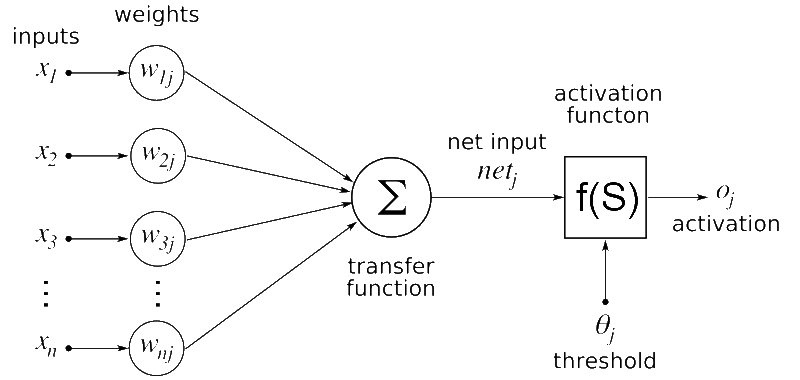
\includegraphics[width=0.8\textwidth]{Figure2-1.png}
\caption{\label{fig:perceptron}Diagram of a perceptron.}
\end{figure}


Each output is updated according to the equation:
\begin{equation}\label{eq:BasicEq}
y_{i} = f(h_{i}) = f\left(\sum_{j}w_{ij}x_{j}\right)
\end{equation}
where $y_{i}$ is the $i$th output, $h_{i}$ is the net input into node $i$, The weight $w_{ij}$ connects the $i$th output and the $j$th input, and $x_{j}$ is the $j$th input. The function $f(h)$ is the activation function and usually makes up the form
\begin{equation}\label{eq:FullEq}
f(h) = sign(h) = 
  \begin{cases}
    -1       & \quad h < 0 \\
    1  & \quad h \geq 0\\
  \end{cases}
\end{equation}
We can also represent \ref{eq:FullEq} in vector notation, as in 
\begin{equation}\label{eq:UsedEq}
y = f(h) = f(\bf w \cdot x)
\end{equation}
where \textbf{w} and \textbf{x} can be regarded as $nx1$ dimensional column vectors, and $n$ is the number of input data.
The term $w \cdot x$ in \ref{eq:UsedEq} constructs a $(n-1)$-dimension hyperplane which passes the origin. The hyperplane can be shifted by adding an parameter to \ref{eq:BasicEq}, for example
\begin{equation}\label{eq:WithBias}
y = f(h) = f(\bf w \cdot x + b)
\end{equation}
We can have the same effect by putting a constant value $1$ and increase the size of $x$ and $w$ by one. The extra weight $w$ with fixed value 1 is called \textit{bias weight}; it is adaptive like other weights and provides flexibility to hyperplane. Then we get:
\begin{equation}\label{eq:finalEq}
y = f(h) = f(\sum_{i=0}^{n}w_{i}x_{i})
\end{equation}
The aim of learning is to find a set of weights $w_{i}$ so that:
\begin{align*}
y = f(\sum_{i=0}^{n}w_{i}x_{i}) = 1  & \quad x \in Class A\\
y = f(\sum_{i=0}^{n}w_{i}x_{i}) = 0  & \quad x \in Class B
\end{align*}


\section{Multi-Layer Networks}

Single-layer networks have some important limitation in terms of the representing range of functions. We are seeking to learn the nonlinearity as the linear discriminant.To improve the representation capability, we can stack layers networks. This is the approach of multilayer neural networks. Multilayer neural networks implement linear discriminants via mapping input data to a nonlinear space. They can use fairly simple algorithms to learn form of the nonlinearity from training data.

In the thesis, we limit multi-layer networks in subset of feedforward networks. As feedforward networks can provide a general mechanism for representing nonlinear functional mapping between a set of input data and a set of labels. The \ref{fig:ffnet} is a feedforward network having two layers of adaptive weights.
\begin{figure}
\centering
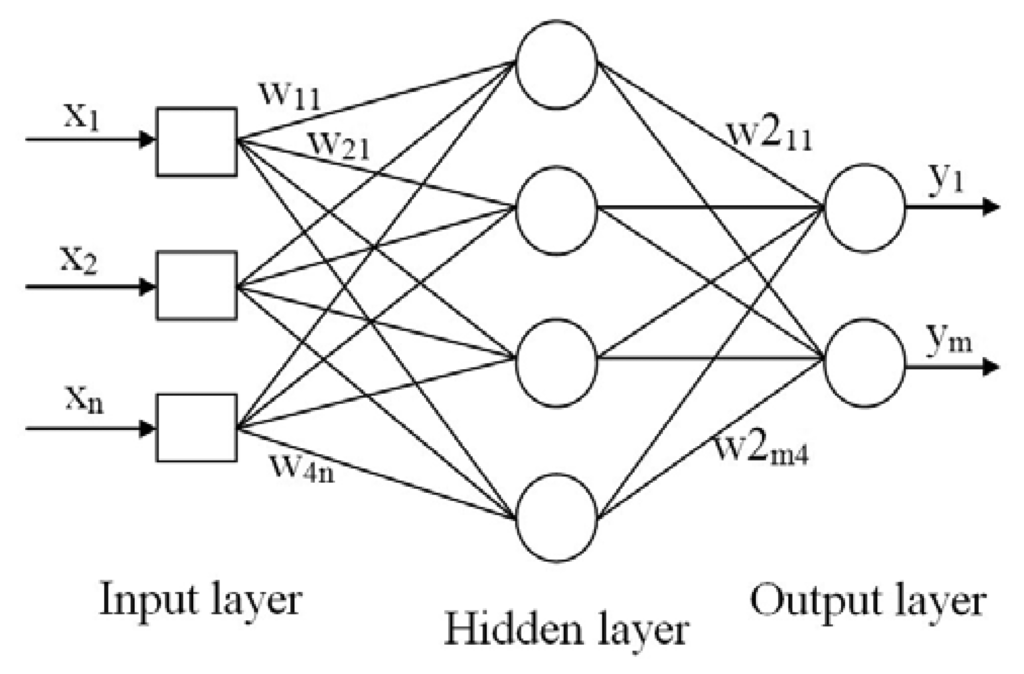
\includegraphics[width=0.8\textwidth]{Figure2-2.png}
\caption{\label{fig:ffnet}Diagram of a feedford neural networks.}
\end{figure}
In the example, the middle column perceptrons act as hidden units. The network has $n$ inputs, $4$ hidden units and $m$ output units. The network diagram represents the function in the form
\begin{equation}\label{eq:ffEq}
y_{m} = \hat{f}\Big(\sum_{j=0}^{m}w_{j4}^{(2)}f\big(\sum_{i=0}^{n}w_{4i}^{(1)}x_{i}\big)\Big)
\end{equation}
In the \ref{eq:ffEq}, outer activation function could be different with the inner one.

There are some choices for activation functions, sigmoid and tanh are related and can provide high capability with continuous input data. Logistic activation function sigmoid can be represented as 
\begin{equation}\label{eq:sigmoid}
f(x) = \frac{1}{1+e^{-x}}
\end{equation}
Its outputs lies in range $(0,1)$. We can do a linear transformation $hat{x}=x/2$ on input data and a linear transformation $hat{y}=2y-1$ on the output. Then we can get an equivalent activation function tanh which can be represented as
\begin{equation}\label{eq:tanh}
f(x) = tanh(x) = \frac{e^{x}-e^{-x}}{e^{x}+e^{-x}}
\end{equation}

The three layer neural network is capable of approximating any function with enough hidden units which means the networks with two layers of weights and sigmoid nonlinearities can provide any accuracy in classification problems. 


\section{Backpropagation}
Multi-layer neural networks can represent mapping from input data to output classes. How to learn a suitable mapping from training dataset? And there is no explicit mapping between output and hidden units. This will be resolved by backpropagation training protocol.

Because networks have differentiable activation functions, the activation of output units can be propagated to hidden units with regard to weights and bias. If we have an error function, we can evaluate derivatives of the error and update the weights to minimize the error function via some optimization methods.

Backpropagation can be applied to find the derivatives of an error function related to the weights and biases in the network via two stages. First, the derivatives of the error functions, for instance sum-of-squares and Jacobian, with respect to the weights must be evaluated. Second, a variety of optimization schemes can be implemented to compute the adjustment of weights based on derivatives. After putting data forward propagation through the network, we can get the output result. It updates weight changes based on grandient descent. The update equation can be represented as
\begin{equation}\label{eq:UpdateWeights}
w(m+1) = w(m) + \Delta w(m)
\end{equation}
where $\Delta w(m)$ defined as 
\begin{equation}\label{eq:DeltaWeights}
\Delta w(m) = -\eta \frac{\partial E}{\partial w}
\end{equation}


We can express error function as
\begin{equation}\label{eq:errorfunc}
E^{n} = E^{n}(y_{1},...,y_{c})
\end{equation}

Then, the derivative of $E^{n}$ with respect to some weights $w_{ji}$ can be calculated and apply chain rule for partial derivatives
\begin{equation}\label{eq:chainrule}
\frac{\partial E^{n}}{\partial w_{ji}} = \frac{\partial E^{n}}{\partial a_{j}} \frac{\partial a_{j}}{\partial w_{ji}} = \delta_{j} \frac{\partial a_{j}}{\partial w_{ji}}
\end{equation}
where $a_{j}$ is the summed inputs to unit $j$ and $\delta_{j}$ is the learning rate. The 
\begin{equation}\label{eq:sensitive}
\delta_{j} = \frac{\partial E^{n}}{\partial a_{ji}}
\end{equation}






\section{Weather Classification}

Weather classification is an important job in daily life. In this thesis, we are focused on two class weather conditions, sunny and cloudy. 

There are some obstacles in front of weather classification. First, because inputting pixels are independent and high dimension, say a 500x500 RPG image means 750000 pixels, computation is huge. Second, some simple middle level image characters are difficult to machines, like light, shading, sun shine. It is still not easy to detect these characters with high accuracy.  Thirdly, there are no decisive features, for example brightness and lightness, to classify scene. For example, sun shine can be both found in sunny and cloudy weather. Last but not least, outdoor images are various background.


